\documentclass{capstonedoc}

% Document Info
\title{VGA Colour Palette Shifter}
\date{2016-03-14}
\author{Stefan Martynkiw}

\usepackage{tikz-timing}
\usetikztiminglibrary[rising arrows]{clockarrows}

\usepackage{cite}
\usepackage[hyphens]{url}

\usepackage{graphicx}
\graphicspath{ {images/} }

\usepackage{caption}

% Macro from http://nathantypanski.com/blog/2014-10-29-tikz-timing.html
\usepackage{xparse} % NewDocumentCommand, IfValueTF, IFBooleanTF

% Reference a bus.
%
% Usage:
%
%     \busref[3::0]{C/BE}    ->   C/BE[3::0]
%     \busref*{AD}           ->   AD#
%     \busref*[3::0]{C/BE}   ->   C/BE[3::0]#
%
\NewDocumentCommand{\busref}{som}{\texttt{%
#3%
\IfValueTF{#2}{[#2]}{}%
\IfBooleanTF{#1}{\#}{}%
}}

\begin{document}
\maketitle
%Document body

\section{Introduction}

With the SRAM containing 8-bit-wide words, it is occaisionally desired to have
graphical output with an increased colour depth. This block allows you to
specify a transition between an 8-bit colour value and an RGB565 output value.
This block contains a 2**8 = 256 byte deep palette ram, which performs a colour
translation when required.

In QSYS, this block slots in between the Video FB streamer (which pulls out
data from the SRAM) and the Video RGB resampler. 

\section{Clocking}

The Colour Palette Shifter runs on the same video clock as the VGA pixel buffer
discussed in our team's other application note.

\section{Interfaces}

The interfaces used for this block are shown in the block diagram below.

\begin{figure}[ht]
  \centering
  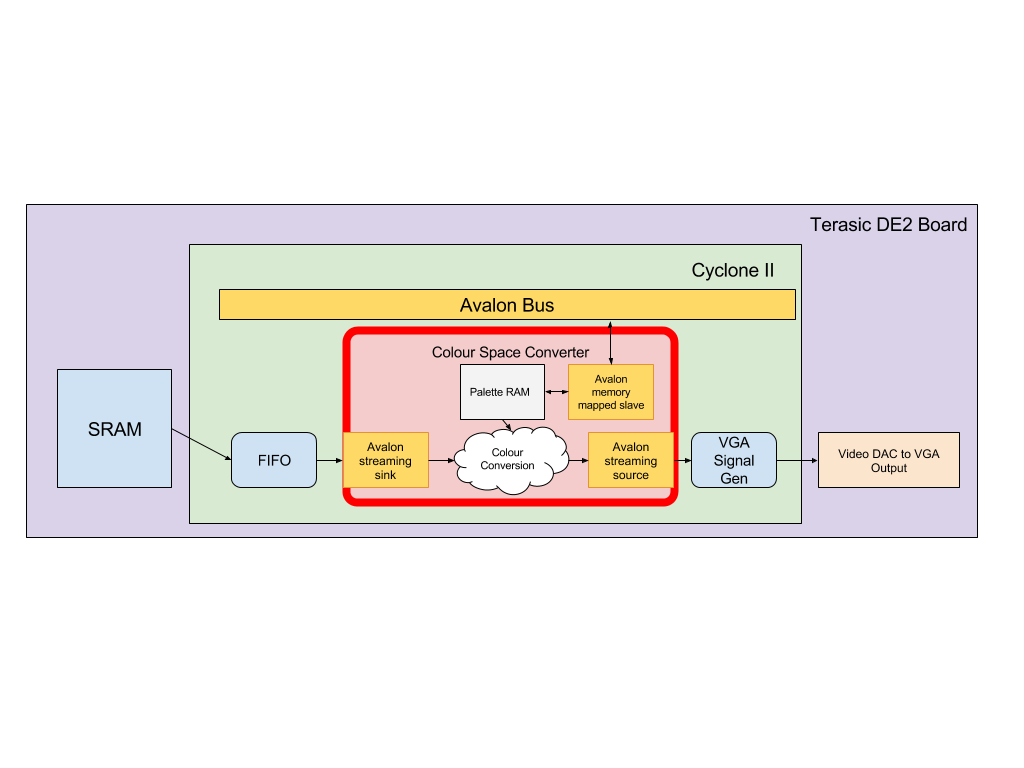
\includegraphics[width=11cm]{block-diagram-design}
  \caption{Block Diagram for Qsys Block}
  \label{fig:blockdiag}
\end{figure}


\section{Avalon-ST}

Avalon-ST is the interface used for streaming data between components. This is
the name of the interface that connects the video output components in the
provided example Qsys system.

This bus consists of a data signal, as well as several control signals. The
interface is not bi-directional, and must flow from source to sink.

For video data as we are using it, the Avalon-ST bus must be clocked at the
same rate as the VGA pixel clock: 25.2MHz. Each clock cycle, a pixel is
transferred over the \texttt{data} signal. The first pixel in a frame is
transmitted with the \texttt{startofpacket} control signal asserted. Likewise,
the final pixel in a frame is transmitted with the \texttt{endofpacket} control
signal asserted. The sink will assert \texttt{ready} when it is able to accept
new pixel data. In the case of a VGA video signal, \texttt{ready} is asserted
while pixels are being output to the display, and is de-asserted during the
VGA blanking period.
The \texttt{valid} control signal is asserted by the source when its data is
ready to send. The Altera-provided video blocks expect this signal to always
be asserted.

In figure~\ref{fig:avalonsttiming}, the end of transmitting a video frame is
shown, with the last several pixels being transmitted, and then the first pixel
of the following frame being sent, at which point the VGA controller begins a
blanking period. Note that the next \texttt{data} value must be available before
\texttt{ready} is asserted again.

\begin{figure}[ht]
\begin{tikztimingtable}[%
    timing/dslope=0.1,
    timing/.style={x=5ex,y=2ex},
    x=5ex,
    timing/rowdist=3ex,
    timing/name/.style={font=\sffamily\scriptsize}
  ]
  \busref{clk}           & 22{c} \\
  \busref{ready}         & 1u 1L 8H 1L 1u \\
  \busref{valid}         & 11H \\
  \busref{data[7:0]}     & 1u 1D{$d_{n-7}$} 1D{$d_{n-6}$} 1D{$d_{n-5}$} 1D{$d_{n-4}$} 1D{$d_{n-3}$} 1D{$d_{n-2}$} 1D{$d_{n-1}$} 1D{$d_n$} 1D{$d_0$} 1D{$d_1$} 1u \\
  \busref{startofpacket} & 1u 8L 1H 1L 1u \\
  \busref{endofpacket}   & 1u 7L 1H 2L 1u \\
  \extracode
  \begin{pgfonlayer}{background}
    \begin{scope}[semitransparent, semithick]
      \vertlines[darkgray,dotted]{0.5, 1.5,...,11.0}
    \end{scope}
  \end{pgfonlayer}
\end{tikztimingtable}
\caption{Avalon-ST Timing Diagram}
\label{fig:avalonsttiming}
\end{figure}

\section{Memory}

The color palette shifter contains an instatiated dual port RAM. This dual-port
RAM has one port attached as an Avalon slave, allowing the user to edit the 
palette. The other port of the RAM is attached to signals which are used in the
state-machine that operates on the Avalon-ST bus in this block. 

The addressing scheme for the palette is very simple. The 8-bit SRAM data "I",
corresponds to an 8-bit address, which returns a 2-byte RGB565 value from 
dual\_port[I].

\section{Project Setup}

The following sections detail how to configure a project using the provided
video blocks.

\subsection{Qsys}

The QSYS configuration of this block follows the vga_pix_buf configuration. 
Between the video\_fb\_streamer and the video\_rgb\_sampler, the colour palette
shifter is added, as shown in the figure below.

\begin{figure}[ht]
  \centering
  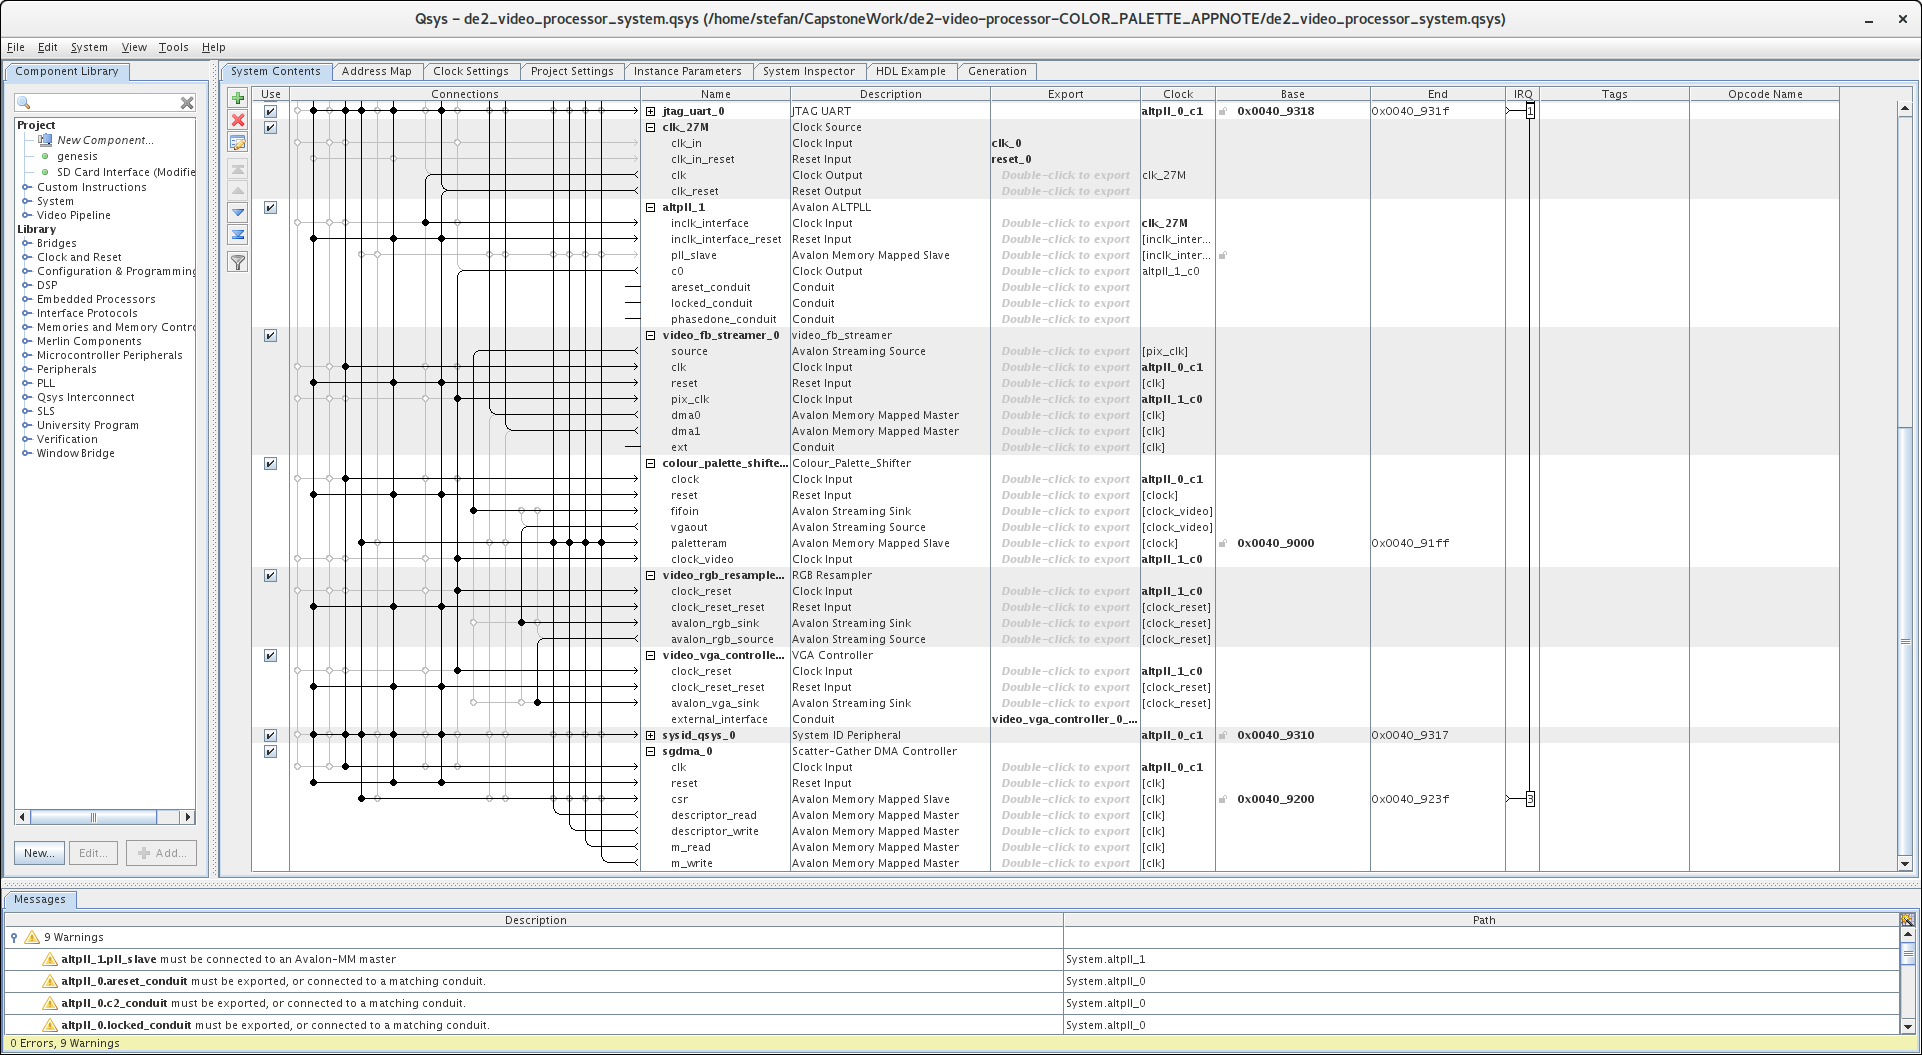
\includegraphics[width=11cm]{qsys_2}
  \caption{Colour Palette Shifter in QSYS system.}
  \label{fig:qsys_2}
\end{figure}

The Colour Palette Shifter Block is configured as shown in the following
screenshots.

\begin{figure}[ht]
  \centering
  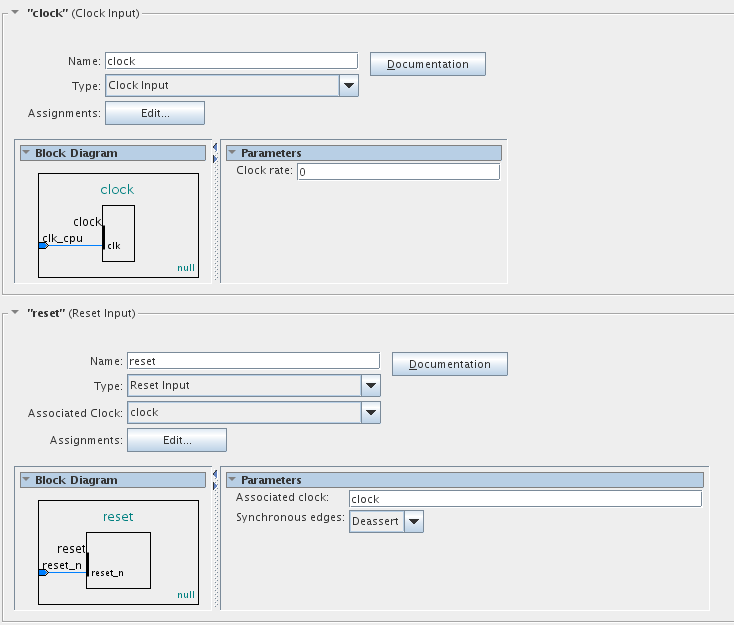
\includegraphics[width=7cm]{qsys_i_1}
  \caption{Configuration for \texttt{Colour\_Space\_Converter}}
  \label{fig:qsysvidfbcfg}
\end{figure}

\begin{figure}[ht]
  \centering
  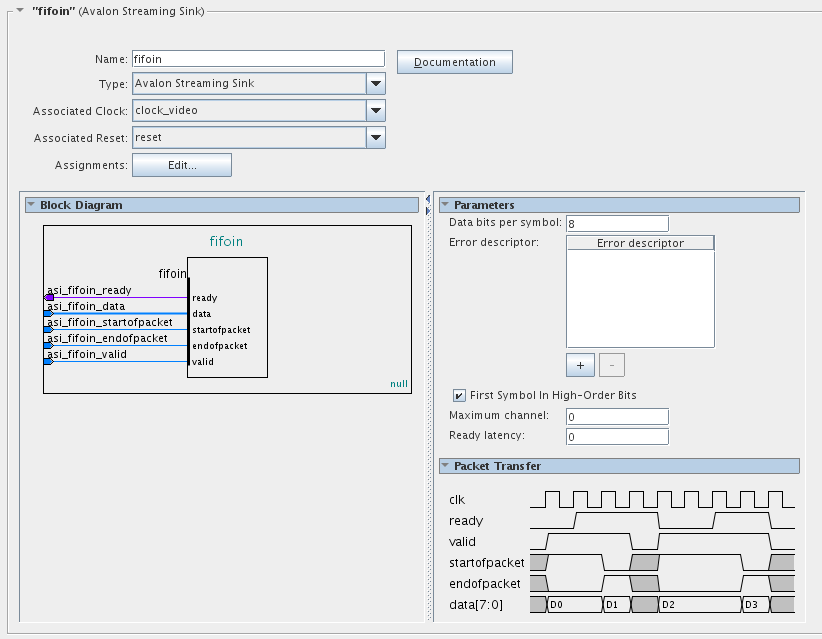
\includegraphics[width=7cm]{qsys_i_2}
  \caption{Configuration for \texttt{Colour\_Space\_Converter}}
  \label{fig:qsysvidfbcfg}
\end{figure}

\begin{figure}[ht]
  \centering
  \includegraphics[width=7cm]{qsys_i_3}
  \caption{Configuration for \texttt{Colour\_Space\_Converter}}
  \label{fig:qsysvidfbcfg}
\end{figure}

\begin{figure}[ht]
  \centering
  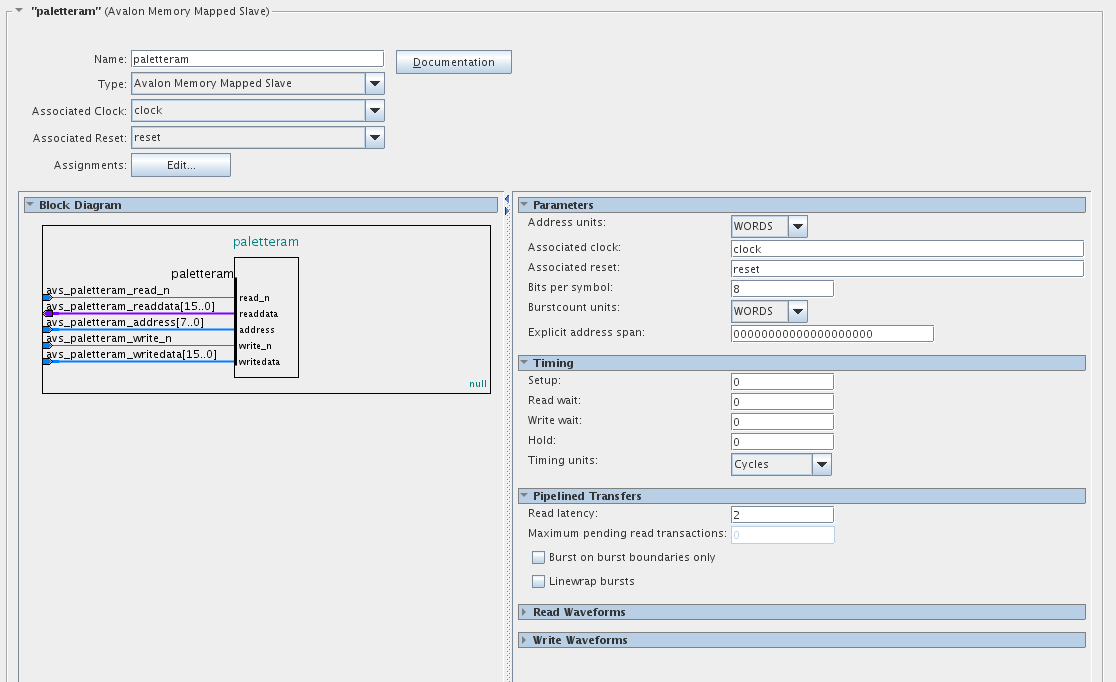
\includegraphics[width=7cm]{qsys_i_4}
  \caption{Configuration for \texttt{Colour\_Space\_Converter}}
  \label{fig:qsysvidfbcfg}
\end{figure}

\begin{figure}[ht]
  \centering
  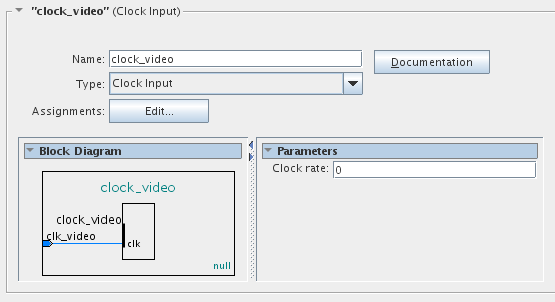
\includegraphics[width=7cm]{qsys_i_5}
  \caption{Configuration for \texttt{Colour\_Space\_Converter}}
  \label{fig:qsysvidfbcfg}
\end{figure}

Finally, the configuration for the \texttt{video\_rgb\_resampler} is shown
in figure~\ref{fig:qsysrgbcfg}. This block must be configured to go from
16-bit colour to 30-bit colour, to match the interfaces of the
\texttt{colour\_space\_converter} and the \texttt{video\_vga\_controller}.


\subsection{Quartus}

You can use the Qsys-provided VHDL template to instantiate your system. This
might look something like Listing~\ref{lst:toplevel} below.

\begin{lstlisting}[language=vhdl,caption={Sample Top Level VHDL File},label={lst:toplevel},tabsize=1]
LIBRARY ieee;
USE ieee.std_logic_1164.all;

ENTITY vga_pix_buffer IS
	PORT
	(
		-- Clocks
		CLOCK_50     : in       std_logic;
		CLOCK_27     : in       std_logic;

		-- SDRAM on board
		DRAM_ADDR    : out      std_logic_vector (11 downto 0);
		DRAM_BA_0    : out      std_logic;
		DRAM_BA_1    : out      std_logic;
		DRAM_CAS_N   : out      std_logic;
		DRAM_CKE     : out      std_logic;
		DRAM_CLK     : out      std_logic;
		DRAM_CS_N    : out      std_logic;
		DRAM_DQ      : inout    std_logic_vector (15 downto 0);
		DRAM_LDQM    : out      std_logic;
		DRAM_UDQM    : out      std_logic;
		DRAM_RAS_N   : out      std_logic;
		DRAM_WE_N    : out      std_logic;

		-- SRAM on board
		SRAM_ADDR    : out      std_logic_vector (17 downto 0);
		SRAM_DQ      : inout    std_logic_vector (15 downto 0);
		SRAM_WE_N    : out      std_logic;
		SRAM_OE_N    : out      std_logic;
		SRAM_UB_N    : out      std_logic;
		SRAM_LB_N    : out      std_logic;
		SRAM_CE_N    : out      std_logic;

		-- VGA output
		VGA_R        : out      std_logic_vector (9 downto 0);
		VGA_G        : out      std_logic_vector (9 downto 0);
		VGA_B        : out      std_logic_vector (9 downto 0);
		VGA_CLK      : out      std_logic;
		VGA_BLANK    : out      std_logic;
		VGA_HS       : out      std_logic;
		VGA_VS       : out      std_logic;
		VGA_SYNC     : out      std_logic;

		-- Input buttons
		KEY          : in       std_logic_vector (3 downto 0)
	);
END ENTITY vga_pix_buffer;

ARCHITECTURE arch OF vga_pix_buffer IS

	COMPONENT vga_pix_buffer_system IS
		PORT (
			clk_50_clk                  : in    std_logic           := 'X';
			reset_50_reset_n            : in    std_logic           := 'X';
			clk_27_clk                  : in    std_logic           := 'X';
			reset_27_reset_n            : in    std_logic           := 'X';
			sram_0_external_interface_DQ                    : inout std_logic_vector(15 downto 0) := (others => 'X');
			sram_0_external_interface_ADDR                  : out   std_logic_vector(17 downto 0);
			sram_0_external_interface_LB_N                  : out   std_logic;
			sram_0_external_interface_UB_N                  : out   std_logic;
			sram_0_external_interface_CE_N                  : out   std_logic;
			sram_0_external_interface_OE_N                  : out   std_logic;
			sram_0_external_interface_WE_N                  : out   std_logic;
			video_vga_controller_0_external_interface_CLK   : out   std_logic;
			video_vga_controller_0_external_interface_HS    : out   std_logic;
			video_vga_controller_0_external_interface_VS    : out   std_logic;
			video_vga_controller_0_external_interface_BLANK : out   std_logic;
			video_vga_controller_0_external_interface_SYNC  : out   std_logic;
			video_vga_controller_0_external_interface_R     : out   std_logic_vector(9 downto 0);
			video_vga_controller_0_external_interface_G     : out   std_logic_vector(9 downto 0);
			video_vga_controller_0_external_interface_B     : out   std_logic_vector(9 downto 0);
			sdram_0_wire_addr                               : out   std_logic_vector(11 downto 0);
			sdram_0_wire_ba                                 : out   std_logic_vector(1 downto 0);
			sdram_0_wire_cas_n                              : out   std_logic;
			sdram_0_wire_cke                                : out   std_logic;
			sdram_0_wire_cs_n                               : out   std_logic;
			sdram_0_wire_dq                                 : inout std_logic_vector(15 downto 0) := (others => 'X');
			sdram_0_wire_dqm                                : out   std_logic_vector(1 downto 0);
			sdram_0_wire_ras_n                              : out   std_logic;
			sdram_0_wire_we_n                               : out   std_logic;
			altpll_sys_dram_c0_clk                          : out   std_logic
		);
	END COMPONENT vga_pix_buffer_system;

	-- Signals to interface with DRAM
	SIGNAL BA   : std_logic_vector (1 downto 0);
	SIGNAL DQM  : std_logic_vector (1 downto 0);

BEGIN

	DRAM_BA_1 <= BA(1);
	DRAM_BA_0 <= BA(0);

	DRAM_UDQM <= DQM(1);
	DRAM_LDQM <= DQM(0);

	sys0 : COMPONENT vga_pix_buffer_system
		PORT MAP (
			clk_50_clk                                      => CLOCK_50,
			reset_50_reset_n                                => KEY(0),
			clk_27_clk                                      => CLOCK_27,
			reset_27_reset_n                                => KEY(0),
			sram_0_external_interface_DQ                    => SRAM_DQ,
			sram_0_external_interface_ADDR                  => SRAM_ADDR,
			sram_0_external_interface_LB_N                  => SRAM_LB_N,
			sram_0_external_interface_UB_N                  => SRAM_UB_N,
			sram_0_external_interface_CE_N                  => SRAM_CE_N,
			sram_0_external_interface_OE_N                  => SRAM_OE_N,
			sram_0_external_interface_WE_N                  => SRAM_WE_N,
			video_vga_controller_0_external_interface_CLK   => VGA_CLK,
			video_vga_controller_0_external_interface_HS    => VGA_HS,
			video_vga_controller_0_external_interface_VS    => VGA_VS,
			video_vga_controller_0_external_interface_BLANK => VGA_BLANK,
			video_vga_controller_0_external_interface_SYNC  => VGA_SYNC,
			video_vga_controller_0_external_interface_R     => VGA_R,
			video_vga_controller_0_external_interface_G     => VGA_G,
			video_vga_controller_0_external_interface_B     => VGA_B,
			sdram_0_wire_addr                               => DRAM_ADDR,
			sdram_0_wire_ba                                 => BA,
			sdram_0_wire_cas_n                              => DRAM_CAS_N,
			sdram_0_wire_cke                                => DRAM_CKE,
			sdram_0_wire_cs_n                               => DRAM_CS_N,
			sdram_0_wire_dq                                 => DRAM_DQ,
			sdram_0_wire_dqm                                => DQM,
			sdram_0_wire_ras_n                              => DRAM_RAS_N,
			sdram_0_wire_we_n                               => DRAM_WE_N,
			altpll_sys_dram_c0_clk                          => DRAM_CLK
		);

END ARCHITECTURE arch;
\end{lstlisting}

\subsection{Nios II SBT for Eclipse}

This section is identical to the vga_pixbuf application note as this application
note extends the previous one.

When you create a new ``Nios II Application and BSP from Template'' project in
Eclipse, you must manually configure the memory map used in the BSP project.
This configuration is shown in figure~\ref{fig:bspconfig}. In particular note
the definitions for \texttt{sdram\_video\_0} and \texttt{sdram\_sys\_0}. This
must match your planned memory layout. If you compare the memory addresses in
figure~\ref{fig:bspconfig} and the \texttt{SDRAM\_VIDEO\_OFFSET} value in the
sample code in Listing~\ref{lst:movinglinecode}, they should refer to the same
location in memory.

\begin{figure}[ht]
  \centering
  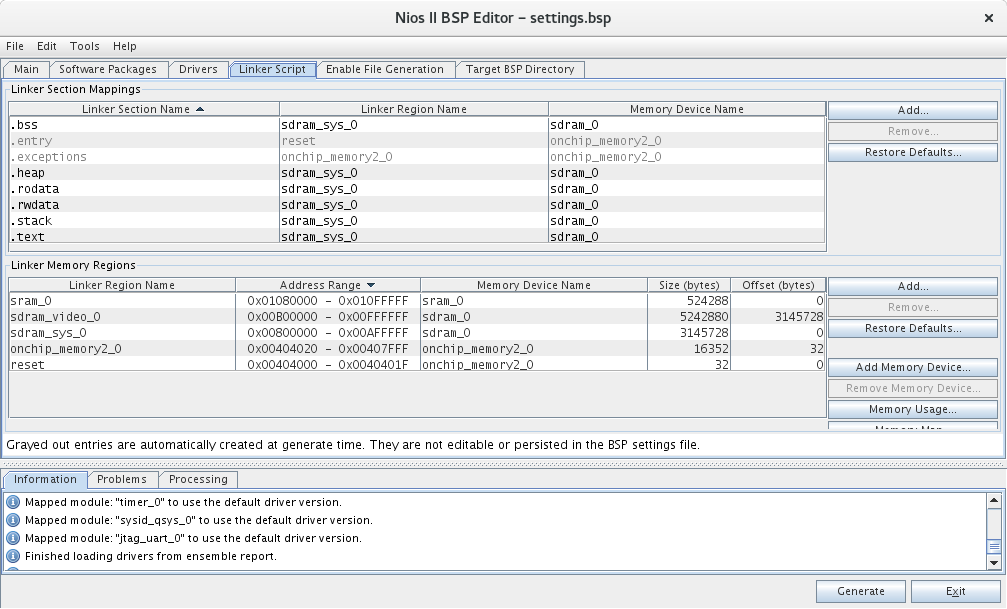
\includegraphics[width=9cm]{bsp_config}
  \caption{BSP Linker Configuration}
  \label{fig:bspconfig}
\end{figure}

\section{Sample Code}

The following code draws a test palette, switches some 

\begin{lstlisting}[language=c,caption={Sample Program that Generates a Test Pattern, then changes the color},label={lst:testcode},tabsize=2]
#include <stdio.h>
#include <io.h>
#include <system.h>
#include <sys/alt_stdio.h>
#include <string.h>

unsigned int palette_ega[16] =
		/* EGA Colour Palette */
		/* Black			  Blue	       Green       Cyan          Red */
		{/*00*/ 0x0000, /*01*/0x0015, /*02*/0x2704, /*03*/0x1E79, /*04*/0xA800,
		 /*     Magenta       Brown   Light Grey     Dark Grey   Bright Blue*/
		 /*05*/ 0xA815, /*06*/0xE3C1, /*07*/0xAD55, /*08*/0x52AA, /*09*/0x52BF,
		 /* BGreen            BCyan         Bred       B Magenta     B Yellow*/
		 /*10*/ 0x57EA, /*11*/0x57FF, /*12*/0xFAAA, /*13*/0xFABF, /*14*/0xFFEA,
		 0xFFFF /*B White */
		};

unsigned int palette_stephen[256] =
		/* Stephen's RGB323 -> RGB565 Palette */
		{0x0 , 0xa , 0x15 , 0x1f , 0x120 , 0x12a , 0x135 , 0x13f , 0x240 ,
		0x24a , 0x255 , 0x25f , 0x360 , 0x36a , 0x375 , 0x37f , 0x480 ,
		0x48a , 0x495 , 0x49f , 0x5a0 , 0x5aa , 0x5b5 , 0x5bf , 0x6c0 ,
		0x6ca , 0x6d5 , 0x6df , 0x7e0 , 0x7ea , 0x7f5 , 0x7ff , 0x2000 ,
		0x200a , 0x2015 , 0x201f , 0x2120 , 0x212a , 0x2135 , 0x213f , 0x2240 ,
		0x224a , 0x2255 , 0x225f , 0x2360 , 0x236a , 0x2375 , 0x237f , 0x2480 ,
		0x248a , 0x2495 , 0x249f , 0x25a0 , 0x25aa , 0x25b5 , 0x25bf , 0x26c0 ,
		0x26ca , 0x26d5 , 0x26df , 0x27e0 , 0x27ea , 0x27f5 , 0x27ff , 0x4800 ,
		0x480a , 0x4815 , 0x481f , 0x4920 , 0x492a , 0x4935 , 0x493f , 0x4a40 ,
		0x4a4a , 0x4a55 , 0x4a5f , 0x4b60 , 0x4b6a , 0x4b75 , 0x4b7f , 0x4c80 ,
		0x4c8a , 0x4c95 , 0x4c9f , 0x4da0 , 0x4daa , 0x4db5 , 0x4dbf , 0x4ec0 ,
		0x4eca , 0x4ed5 , 0x4edf , 0x4fe0 , 0x4fea , 0x4ff5 , 0x4fff , 0x6800 ,
		0x680a , 0x6815 , 0x681f , 0x6920 , 0x692a , 0x6935 , 0x693f , 0x6a40 ,
		0x6a4a , 0x6a55 , 0x6a5f , 0x6b60 , 0x6b6a , 0x6b75 , 0x6b7f , 0x6c80 ,
		0x6c8a , 0x6c95 , 0x6c9f , 0x6da0 , 0x6daa , 0x6db5 , 0x6dbf , 0x6ec0 ,
		0x6eca , 0x6ed5 , 0x6edf , 0x6fe0 , 0x6fea , 0x6ff5 , 0x6fff , 0x9000 ,
		0x900a , 0x9015 , 0x901f , 0x9120 , 0x912a , 0x9135 , 0x913f , 0x9240 ,
		0x924a , 0x9255 , 0x925f , 0x9360 , 0x936a , 0x9375 , 0x937f , 0x9480 ,
		0x948a , 0x9495 , 0x949f , 0x95a0 , 0x95aa , 0x95b5 , 0x95bf , 0x96c0 ,
		0x96ca , 0x96d5 , 0x96df , 0x97e0 , 0x97ea , 0x97f5 , 0x97ff , 0xb000 ,
		0xb00a , 0xb015 , 0xb01f , 0xb120 , 0xb12a , 0xb135 , 0xb13f , 0xb240 ,
		0xb24a , 0xb255 , 0xb25f , 0xb360 , 0xb36a , 0xb375 , 0xb37f , 0xb480 ,
		0xb48a , 0xb495 , 0xb49f , 0xb5a0 , 0xb5aa , 0xb5b5 , 0xb5bf , 0xb6c0 ,
		0xb6ca , 0xb6d5 , 0xb6df , 0xb7e0 , 0xb7ea , 0xb7f5 , 0xb7ff , 0xd800 ,
		0xd80a , 0xd815 , 0xd81f , 0xd920 , 0xd92a , 0xd935 , 0xd93f , 0xda40 ,
		0xda4a , 0xda55 , 0xda5f , 0xdb60 , 0xdb6a , 0xdb75 , 0xdb7f , 0xdc80 ,
		0xdc8a , 0xdc95 , 0xdc9f , 0xdda0 , 0xddaa , 0xddb5 , 0xddbf , 0xdec0 ,
		0xdeca , 0xded5 , 0xdedf , 0xdfe0 , 0xdfea , 0xdff5 , 0xdfff , 0xf800 ,
		0xf80a , 0xf815 , 0xf81f , 0xf920 , 0xf92a , 0xf935 , 0xf93f , 0xfa40 ,
		0xfa4a , 0xfa55 , 0xfa5f , 0xfb60 , 0xfb6a , 0xfb75 , 0xfb7f , 0xfc80 ,
		0xfc8a , 0xfc95 , 0xfc9f , 0xfda0 , 0xfdaa , 0xfdb5 , 0xfdbf , 0xfec0 ,
		0xfeca , 0xfed5 , 0xfedf , 0xffe0 , 0xffea , 0xfff5 , 0xffff };

unsigned int palette_magenta[256] = {0xA815};

unsigned int bunch_o_blues[256] = {0x000 , 0x001 , 0x002 , 0x003 , 0x004 , 0x005 , 0x006 , 0x007 , 0x008 ,
		0x009 , 0x00a , 0x00b , 0x00c , 0x00d , 0x00e , 0x00f , 0x0010 ,
		0x0011 , 0x0012 , 0x0013 , 0x0014 , 0x0015 , 0x0016 , 0x0017 , 0x0018 ,
		0x0019 , 0x001a , 0x001b , 0x001c , 0x001d , 0x001e , 0x001f };

unsigned int bunch_o_reds[256] = {0x000 , 0x010 , 0x020 , 0x030 , 0x040 , 0x050 , 0x060 , 0x070 , 0x080 ,
		0x090 , 0x0a0 , 0x0b0 , 0x0c0 , 0x0d0 , 0x0e0 , 0x0f0 , 0x0100 ,
		0x0110 , 0x0120 , 0x0130 , 0x0140 , 0x0150 , 0x0160 , 0x0170 , 0x0180 ,
		0x0190 , 0x01a0 , 0x01b0 , 0x01c0 , 0x01d0 , 0x01e0 , 0x01f0};



unsigned int* palettes[6] = {&palette_ega[0], &palette_stephen[0], &palette_magenta[0], &bunch_o_blues[0], &bunch_o_reds[0]};
unsigned int palettes_legnth = 5;



//Make a function to switch the palettes given a pointer to a palette array.
void switchPalette(unsigned int* palette, int length){

	int i = 0;
	for (i = 0; i < length; i++){
		IOWR_16DIRECT(COLOUR_PALETTE_SHIFTER_0_BASE, 2*i, 0x0000);
		IOWR_16DIRECT(COLOUR_PALETTE_SHIFTER_0_BASE, 2*i, palette[i]);
	}


}


void printPalette(int n){
	// Print everything in the palette ram, upto int colours.
	int i;
	unsigned int c;

	unsigned int results[512] = {'\0'};

	for (i = 0; i < n; i++){
		c = IORD_16DIRECT(COLOUR_PALETTE_SHIFTER_0_BASE, 2*i); //offset multiplied by 2 to be on 16-bit boundaries.
		//alt_printf("palette[ %x ]: %x ", 2*i, c);
		results[i] = c;
	}

	for (i = 0; i < n; i++){
		alt_printf("palette[ %x ]: %x ", 2*i, results[i]);
	}

}

int main()
{


	unsigned int row = 0;
	unsigned int col = 0;
	unsigned int delay = 0;

	unsigned int color;
	int i;



	// Clear the screen first.
	alt_putstr("Clear the screen\n");
	for (col = 0; col < 640; col = col + 4){
		for (row = 0; row < 480; row++){
			color = 0;
			IOWR_32DIRECT(SRAM_0_BASE, row * 640 + col, color << 24 | color << 16 | color << 8 | color << 0);
		}
	}


	//Switch palettes here (to EGA colour palette)
	printPalette(16);
	switchPalette(palette_ega, 16);
	printPalette(16);

	alt_putstr("Screen painting demo\n");

	for (i = 0; i < 16; i++){
		alt_printf("Colour");
		for (delay = 0; delay < 700/*2000*/; delay++){
			unsigned int tdelay = delay;
			for (tdelay; tdelay > 0; tdelay--){}
		}

		for (row=0; row<480; row++){
			for (col = 0; col < 640; col=col+4){
				color = i;
				IOWR_32DIRECT(SRAM_0_BASE, row * 640 + col, color << 24 | color << 16 | color << 8 | color << 0);
			}

		}
	}



	alt_putstr("\nStarting Stephen Test Pattern\n");
	int p = 0;
	for (p = 0; p < 8; p++) {

		switchPalette(palettes[p%palettes_legnth], 256);

		alt_putstr("Clear the screen\n");
		for (col = 0; col < 640; col = col + 4){
			for (row = 0; row < 480; row++){
				color = 0;
				IOWR_32DIRECT(SRAM_0_BASE, row * 640 + col, color << 24 | color << 16 | color << 8 | color << 0);
			}
		}


		//Now draw the test pattern
		for (row = 0; row < 480; row++)
		{
			for (col = 0; col < 640; col = col + 4)
			{
				color = ((row + col) % 256) << 0 | ((row + col) % 256) << 8 | ((row + col) % 256) << 16 | ((row + col) % 256) << 24;
				if (row == 0 || row == 479)
				{
					IOWR_32DIRECT(SRAM_0_BASE, row * 640 + col, 0xFFFFFFFF);
				}
				else if (col == 0)
				{
					IOWR_32DIRECT(SRAM_0_BASE, row * 640 + col, 0x000000FF | color);
				}
				else if (col == 636)
				{
					IOWR_32DIRECT(SRAM_0_BASE, row * 640 + col, 0xFF000000 | color);
				}
				else
				{
					IOWR_32DIRECT(SRAM_0_BASE, row * 640 + col, color);
				}
			}
		}


	}





	alt_putstr("Done.\n");


	// Do Stephen's pattern display.

	// And switch the palettes.


  return 0;
}
\end{lstlisting}

%\bibliographystyle{ieeetr}
%\bibliography{vga_color_palette_shifter}

\end{document}
